

\begin{center}
  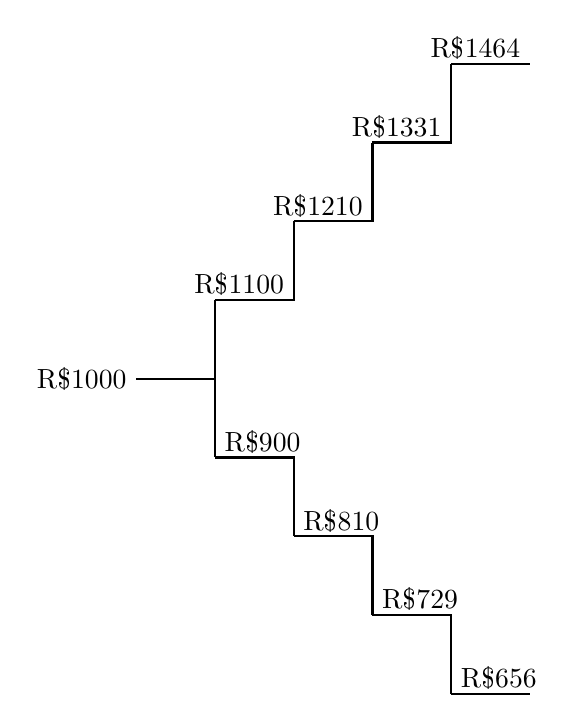
\begin{tikzpicture}{scale = 0.7}
    % Definição dos valores
    \def\valA{R\$1000}
    \def\valB{R\$1100}
    \def\valC{R\$1210}
    \def\valD{R\$1331}
    \def\valE{R\$1464}

    \def\desA{R\$1000}
    \def\desB{R\$900}
    \def\desC{R\$810}
    \def\desD{R\$729}
    \def\desE{R\$656}

    % Degraus da valorização
    \draw[thick] (0,0) -- (1,0) -- (1,1);
    \draw[thick] (1,1) -- (2,1) -- (2,2);
    \draw[thick] (2,2) -- (3,2) -- (3,3);
    \draw[thick] (3,3) -- (4,3) -- (4,4);
    \draw[thick] (4,4) -- (5,4);


    % Degraus da desvalorização
    \draw[thick] (0,0) -- (1,0) -- (1,-1);
    \draw[thick] (1,-1) -- (2,-1) -- (2,-2);
    \draw[thick] (2,-2) -- (3,-2) -- (3,-3);
    \draw[thick] (3,-3) -- (4,-3) -- (4,-4);
    \draw[thick] (4,-4) -- (5,-4);

    % Anotando os valores na valorização
    \node[left] at (0,0) {\valA};
    \node[left] at (2,1.2) {\valB};
    \node[left] at (3,2.2) {\valC};
    \node[left] at (4,3.2) {\valD};
    \node[left] at (5,4.2) {\valE};

    % Anotando os valores na desvalorização
    \node[right] at (1,-0.8) {\desB};
    \node[right] at (2,-1.8) {\desC};
    \node[right] at (3,-2.8) {\desD};
    \node[right] at (4,-3.8) {\desE};
  \end{tikzpicture}
\end{center}
